%%%%%%%%%%%%%%%%%%%%%%%%%%%%%%%%%%%%%%%%%%%%%%%%%%%%%%%%%%%%%%%%%%%%%%%%
% Escuela Politécnica Superior de la Universidad de Alicante
% Realizado por: Jose Manuel Requena Plens
% Contacto: info@jmrplens.com / Telegram:@jmrplens
%%%%%%%%%%%%%%%%%%%%%%%%%%%%%%%%%%%%%%%%%%%%%%%%%%%%%%%%%%%%%%%%%%%%%%%%

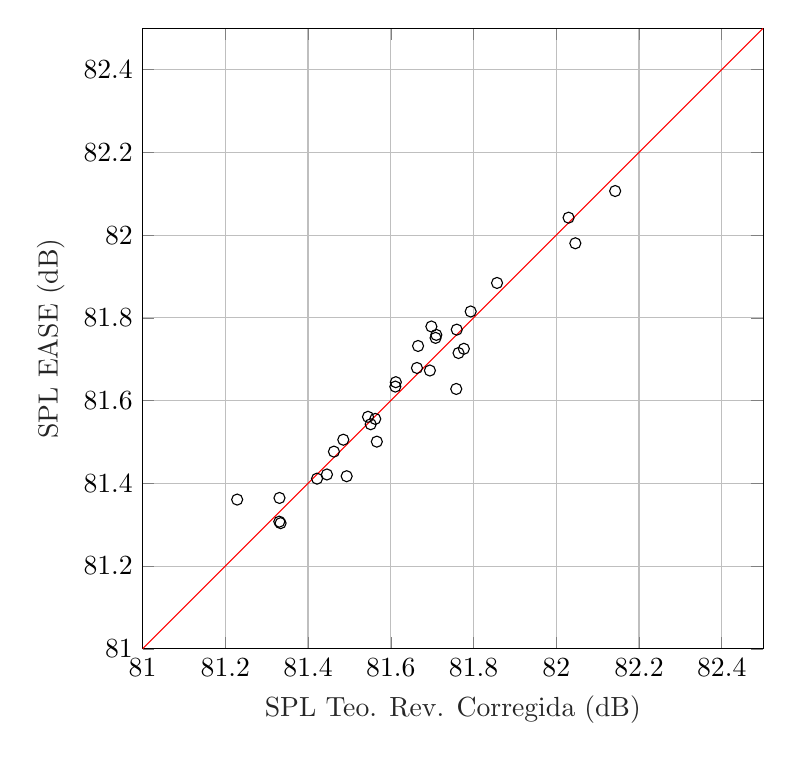
\begin{tikzpicture}

\begin{axis}[%
width=\textwidth,
height=0.65\textwidth,
at={(0\textwidth,0\textwidth)},
scale only axis,
xmin=81,
xmax=82.5,
xlabel style={font=\color{white!15!black}},
xlabel={SPL Teo. Rev. Corregida (dB)},
ymin=81,
ymax=82.5,
axis equal image=true,
%minor x tick num= 1,
%minor y tick num= 1,
%ytick distance=0.1,
ylabel style={font=\color{white!15!black}},
ylabel={SPL EASE (dB)},
axis background/.style={fill=white},
xmajorgrids,
xminorgrids,
ymajorgrids,
yminorgrids,
legend style={legend cell align=left, align=left, draw=white!15!black}
]
\addplot [color=black, only marks, mark=o]
  table[row sep=crcr]{%
81.3305296547238	81.3073310056163\\
81.3309756894275	81.3646161982760\\
81.4217817790589	81.4113118989799\\
81.5514551505769	81.5427746603436\\
81.7637826320174	81.7149648901030\\
81.8568097062743	81.8842901741657\\
82.0297157546384	82.0420758435460\\
82.1423350384191	82.1065076892564\\
82.0460870818860	81.9801976948824\\
81.7931265121477	81.8153278042122\\
81.6121855876210	81.6444437423156\\
81.4456890191893	81.4213603264741\\
81.4625715488726	81.4766294965395\\
81.3336582166581	81.3036744085104\\
81.4933895955345	81.4171803964508\\
81.5624088971591	81.5556673185916\\
81.6945279991275	81.6726539122673\\
81.7082789264959	81.7515321659525\\
81.7594343944194	81.7714425067642\\
81.7766272909335	81.7251289702007\\
81.7582478723122	81.6280859038836\\
81.5662619687015	81.5007217779321\\
81.5449185456124	81.5607325127671\\
81.2287297336981	81.3607141327099\\
81.6632557687887	81.6788248178130\\
81.7100391109355	81.7587706389431\\
81.6981070013399	81.7790120372236\\
81.6659553549367	81.7319709401595\\
81.6110145624761	81.6337827595442\\
81.4852204366460	81.5053942062031\\
};

\addplot [red,samples at={81,82.5}] {x};
\end{axis}
\end{tikzpicture}%